\documentclass[12pt,norsk,a4paper]{article}
\usepackage[norsk]{babel}
\usepackage[norsk]{isodate}
\usepackage[T1]{fontenc}
\usepackage{parskip}
\usepackage{url}
\usepackage{mathtools}
\usepackage{xfrac}
\usepackage{listings}
\author{Frida Berge (fridatbe)}
\title{MAT1120 --- Obligatorisk oppgave 2}
\date{\today}
\usepackage[small,euler-digits]{eulervm}
\usepackage{color}
% \usepackage{minted}
\usepackage{xcolor}
\definecolor{LightGray}{gray}{0.9}
\usepackage{a4wide}
\usepackage[top=2cm]{geometry}
\usepackage{graphicx}
\graphicspath{ {./fig/} }
\newcommand{\tuple}[1]{\ensuremath{\langle #1\rangle}}
\newcommand{\set}[1]{\ensuremath{\{#1\}}}
\newcommand{\imp}{\ensuremath{\rightarrow}}
\newcommand{\M}{\ensuremath{\mathcal{M}}}
\newcommand{\AF}{edge from parent[draw=none]}
\newcommand{\NODE}[1]{\{node \{\ensuremath{#1}\}\}}
\usepackage[explicit]{titlesec}
\titleformat{\section}{\normalfont\Large\bfseries}{}{0em}{#1\ \thesection}


\begin{document}
    \maketitle
    \renewcommand{\thesubsection}{(\alph{subsection})}
    \newpage

    \section{Oppgave}
    \textbf{a)}\\

        Hver av $p(t_i) = s_i$ skal oppfylles og polynomet skal settes opp på formen\\
        $p(t) = c_0 + c_1t + c_2t^2+c_3t^3$\\
        Som kan kan utvides/nøyanseres til:\\
        $p(t) = c_0t^0 + c_1t^1 + c_2t^2+c_3t^3$\\
        Hvis man da betrakter første punkt hvor $t_1 = 2$ og $s_1 = 7$, kan utrykket skrives:\\
        $p(t_1) = c_02^0 + c_12^1 + c_22^2+c_32^3$\\
        $p(t_1) = c_01 + c_12 + c_24+c_38$\\
        Ved å utrykke dette med vektorer:\\
        \[p(t_1)= \left[ \begin{array}{cccc}1 & 2 & 4 & 8\end{array} \right] \left[ \begin{array}{c}c_0 \\ c_1 \\ c_2 \\ c_3\end{array} \right] = 7\]
        Slik kan alle fem likningene settes opp i et likningssystem (med hver søyle tilsvarende ulik grad i polynomene, og hver kolonne tilsvarende ett punkt) og dermed fås utrykket A\textbf{x}=\textbf{b}:\\
        \[A = \left[ \begin{array}{cccc}
                                        1 & 2 & 4 & 8\\
                                        1 & 3 & 9 & 27\\
                                        1 & 4 & 16 & 64\\
                                        1 & 5 & 25 & 125\\
                                        1 & 6 & 36 & 216\\
                                    \end{array} \right]
            \left[ \begin{array}{c}
                                        c_0 \\ 
                                        c_1 \\ 
                                        c_2 \\ 
                                        c_3
                                    \end{array} \right]
            = \left[ \begin{array}{c}
                                        7 \\ 
                                        3 \\ 
                                        5 \\ 
                                        4\\
                                        3
                     \end{array} \right]\]
            


        \textbf{b)}\\\\
        Brukte python (radredukjson.py) til å radredusere den utvidede matrisen (A,b):\\
            \[\left[ \begin{array}{cccc|r}
                1 & 2 & 4 & 8 & 7\\
                1 & 3 & 9 & 27 & 3\\
                1 & 4 & 16 & 64 & 5\\
                1 & 5 & 25 & 125 & 4\\
                1 & 6 & 36 & 216 & 3\\
            \end{array} \right] \texttildelow
            \left[ \begin{array}{cccc|r}
                1 & 0 & 0 & 0 & 0\\
                0 & 1 & 0 & 0 & 0\\
                0 & 0 & 1 & 0 & 0\\
                0 & 0 & 0 & 1 & 0\\
                0 & 0 & 0 & 0 & 1\\
            \end{array} \right]
            \] 
        
        Siden alle søylene er pivotsøyler vil ikke likningssystemet ha noen løsning da det i nederste rad vil gi selvmotsigelsen 
        $0*c_0+0*c_1+0*c_2+0*c_3 = 1$\\
        Koden:\\
        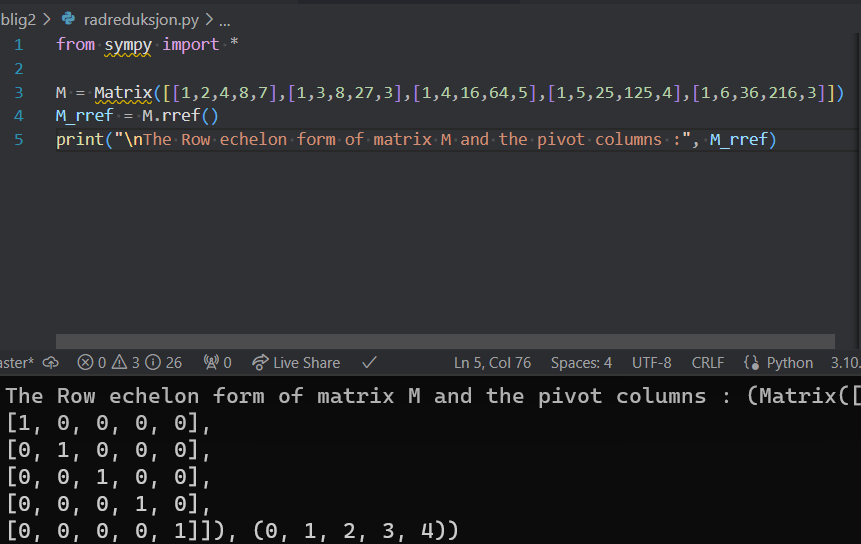
\includegraphics[width=0.6\textwidth]{bilde_kode.png}

        \textbf{c)}\\\\
        Vet fra teorien at det fins et teorem som sier at for å løse aproksimasjonslproblemet: $A\textbf{x}\approx\textbf{b}$
        må man finne en \textbf{x} som gjør avstanden $||\textbf{b}-A\textbf{b}||$ minst mulig.
        Dette vil si at S som er summen av avvikene ($s_1-p(t_i)$ er avstand fra punkt i til grafen til p) skal minimeres.
        Dette kan løses ved å sette opp likningen $(A^TA)\textbf{x}=A^T\textbf{b}$. Siden det er vektoren (matrise med én søyle) \textbf{x} man er ute etter å finne,
        og \textbf{x} består av $c_0, ..., c_3$ vil altså disse koeffisientene $c_i$ finnes ved å løse likningsystemet (1).
        \\
        Likningsystemet (1) vil ha en entydig løsning dersom søylene i matrisen A er lineært uavhengige, som er vist tidligere ved at den kan radreduseres slik at alle de fire søylene inneholder pivotelementer.

        \textbf{d)}\\\\
        Løser likningen\\
        \[(A^TA)\textbf{x}=A^T\textbf{b}\]
        Brukte python til å finne $A^TA$ og $A^T\textbf{b}$\\
        \[\left[ \begin{array}{cccc}
            5 & 20 & 89 & 440\\
            20 & 90 & 437 & 2274\\
            89 & 437 & 2257 & 12173\\
            440 & 2274 & 12173 & 67170\\
        \end{array} \right]
        \left[ \begin{array}{c}
            c_0\\
            c_1\\
            c_2\\
            c_3\\
        \end{array} \right]
        =
        \left[ \begin{array}{c}
            22\\
            81\\
            340\\
            1605\\
        \end{array} \right]\]
        Finner \textbf{x} ved å sette opp en utvidet matrise og radredusere:\\

        Brukte Python til å lage grafen.\\
        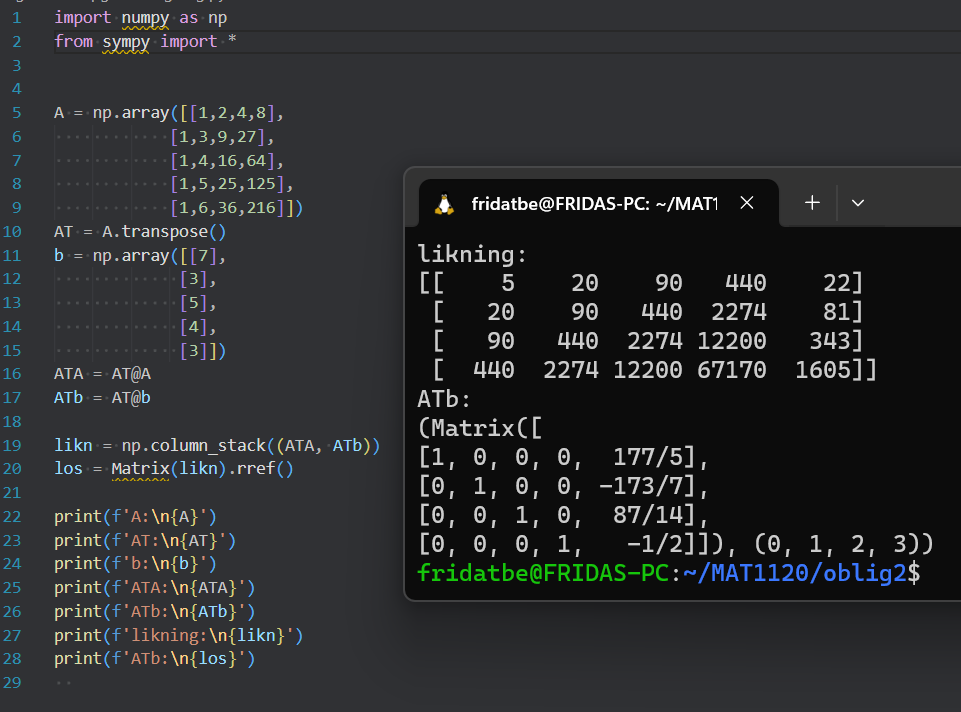
\includegraphics[width=0.5\textwidth]{opg1d_bilde.png}
        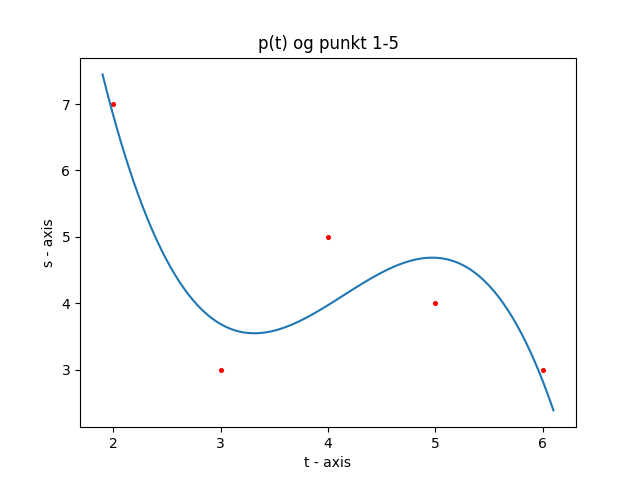
\includegraphics[width=0.5\textwidth]{opg1d.png}\\
        \[\textbf{x} = 
            \left[ \begin{array}{c}
                c_0\\
                c_1\\
                c_2\\
                c_3\\
            \end{array} \right]=
            \left[ \begin{array}{c}
                \frac{177}{5}\\
                -\frac{173}{7}\\
                \frac{87}{14}\\
                -\frac{1}{2}\\
            \end{array} \right]\]


            \textbf{e)}\\\\
        Setter opp den nye likningen:\\
        \[A = \left[ \begin{array}{ccccc}
            1 & 2 & 4 & 8 & 16\\
            1 & 3 & 9 & 27 & 81\\
            1 & 4 & 16 & 64 & 256\\
            1 & 5 & 25 & 125 & 625\\
            1 & 6 & 36 & 216 & 1296\\
        \end{array} \right]
        \left[ \begin{array}{c}
                    c_0 \\ 
                    c_1 \\ 
                    c_2 \\ 
                    c_3 \\
                    c_4
                \end{array} \right]
        = \left[ \begin{array}{c}
                    7 \\ 
                    3 \\ 
                    5 \\ 
                    4 \\
                    3 \\
                \end{array} \right]\]
        Brukte python til å løse likningsystemt og fant løsningen:\\
        \[\textbf{x} = \left[ \begin{array}{c}c_0 \\ c_1 \\ c_2 \\ c_3 \\ c_4 \end{array} \right] = \left[ \begin{array}{c}129 \\ -135 \\ 52 \\ \frac{-17}{2} \\ \frac{1}{2} \end{array} \right]\]

        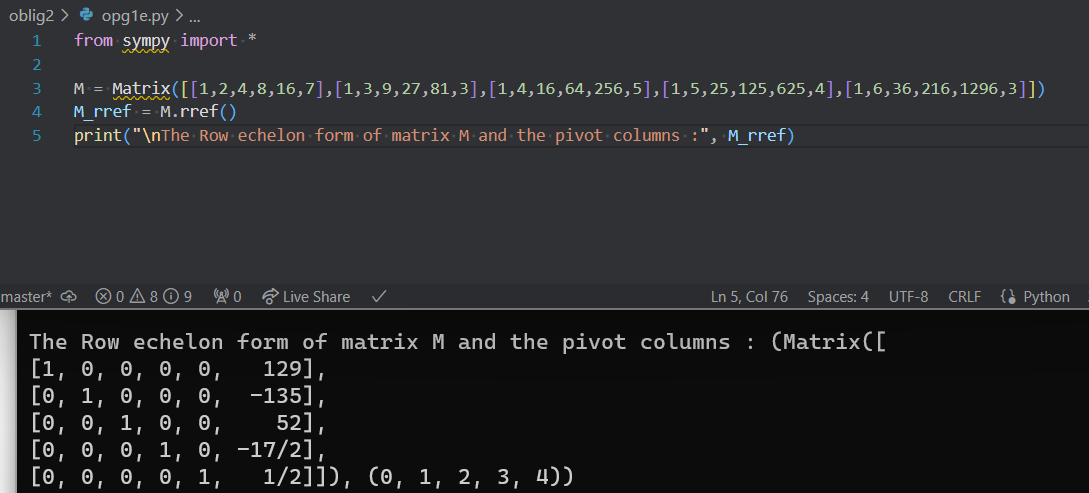
\includegraphics[width=0.6\textwidth]{opg1e.png}\\\\

        \textbf{f)}\\
            Brukte Python til å lage grafen.\\
            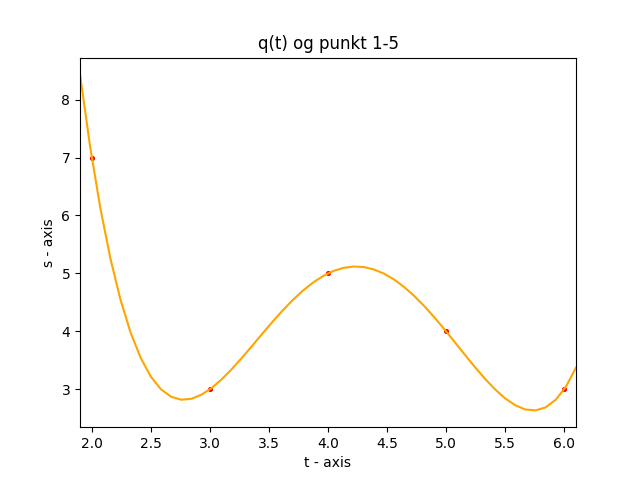
\includegraphics[width=0.6\textwidth]{opg1f.png}\\

        \textbf{g)}\\
            T er en lineærtransformasjon fordi det oppfyller kravene:\\
            \begin{itemize}
                \item $T(p+q) = p+q$\\
                    $T(p+q) = ((p+q)(t_0), (p+q)(t_1), ..., (p+q)(t_n))\\
                    = (p(t_0)+q(t_0), p(t_1)+q(t_1), ..., p(t_n)+q(t_n))\\
                    = (p(t_0), p(t_1), ..., p(t_n))+(q(t_0), q(t_1), ..., q(t_n))\\
                    = \underline{p(t) + q(t)}$
                \item $T(r*p) = r*p$\\
                    $T(r*p) = (r*p(t_0), r*p(t_1),..., r*p(t_n))\\
                    = r(p(t_0), p(t_1), ..., p(t_n))\\
                    = \underline{r*p(t)}$
            \end{itemize}
            Der p og q er polynomer og r er et reelt tall
                
                


        \textbf{h)}\\
            Må vise at $T(p) = \textbf{0}$ bare hvis $p(t_i)$ = 0 for alle $0<=i<=n$\\
            $T(p) = (p(t_0), p(t_1), . . . , p(t_n))$
            Kjernen til T vil være når alle liknignene under oppfylles\\
            \[p(t_0) = d_0t_0^0 + d_1t_0^1 + d_2t_0^2 + ... + d_nt_0^n = 0\]
            \[p(t_1) = d_0t_1^0 + d_1t_1^1 + d_2t_1^2 + ... + d_nt_1^n = 0\]
            \[...\]
            \[p(t_n) = d_0t_n^0 + d_1t_n^1 + d_2t_n^2 + ... + d_nt_n^n = 0\]
            For et polynom p(t) med grad n vil det finnes maksimum n ulike løsninger av  p(t) = 0 (i følge algebraens fundamentalteorem)
            Og siden det er n+1 ulike $p(t_i)$ vil derfor minst én av dem ikke kunne være 0. Derfor står man igjen med at det kun er nullpolynomet
            selv som vil utgjøre Ker(T), fordi uansett hvilken $t_i$ som tas inn i funkjsonen p vil $p(t_i) = 0$
            

        \textbf{i)}\\
        T er isomorfi dersom den er både injektiv og surjektiv.\\
        \begin{itemize}
            \item Injektiv: for at en lineærtransformasjon T skal være én-til-én (injektiv) må Kjernen til T kun bestå av nullvektoren (i følge teorem). Og dette er bevist i forrige oppgave h). Og dermed er T injektiv
            \item Surjektiv: for at en lineærtransformasjon være surjektiv i $P_n -> R^{n+1}$ må det for hver vektor/punkt i $P_n$ finnes minst én vektor/punkt i $R^{n+1}$ som kan nås ved å bruke lineærtransformasjonen på puktet i $P^n$
            Det vil si at hele $R^3$ utsspennes av lineærtransformasjonen T. Siden dimensjonen til lineærtrtransformasjonen er av dimensjon n+1. (fordi det går fra $t_0$ til $t_n$) vil lineærtranformasjonen kunne nå hele $R^{n+1}$
        \end{itemize}


        \textbf{j)}\\
            Kan sette opp systemet med likningene
            \[p(t_0) = d_0t_0^0 + d_1t_0^1 + d_2t_0^2 + ... + d_nt_0^n = 0\]
            \[p(t_1) = d_0t_1^0 + d_1t_1^1 + d_2t_1^2 + ... + d_nt_1^n = 0\]
            \[...\]
            \[p(t_n) = d_0t_n^0 + d_1t_n^1 + d_2t_n^2 + ... + d_nt_n^n = 0\]
            Kan legge likningsystemet i en matrise slik:\\
            \[ T(p) = T(p(t_0), p(t_1), ..., p(t_n)) = \left[ \begin{array}{ccccc}
                1 & t_0 & ... & t_0^{(n)} & s_0\\
                1 & t_1 & ... & t_1^{(n)} & s_1\\
                ... &  &  &  & \\
                1 & t_n & ... & t_n^{(n)} & s_n\\
            \end{array} \right] \]
            Som er en Vandermonde matrise av typen (n x n) * (n x n) og vet derfor fra teorien at dersom alle t-ene er ulike
            vil determinanten ikke kunne være lik 0. Ser derfor på alle søylene uten om siste (som inneholder $s_i$) og vet at
            de vil danne identitestmatrisen ved radreduksjon. Kan derfor sette opp et likningsystsem slik (siden det ikke er noen frie variabler):
            \[d_0*1 + d_1*0 + ... + d_n*0 = c_0\]
            \[d_0*0 + d_1*1 + ... + d_n*0 = c_1\]
            \[...\]
            \[d_0*0 + d_1*0 + ... + d_n*1 = c_n\]
            Der $c_i$ er tallene i søylen lengst til høyre etter at det har blitt utført radreduskjsoner (endringer på $s_i$).
            Som gir verdiene $d_0 = c_0$, $d_1 = c_1$, ..., $d_n = c_n$\\
            Så polynomet p som interpolerer alle punktene $p(t_i)=s_i$ er:\\
            \[p(t) = c_0 + c_1t_n + c_2t_n^2 + ... + c_nt_n^n\]
            

    \newpage


    \section{Oppgave}
    \textbf{a)}\\

    \[\left\langle f,g \right.\rangle=
    \frac{1}{L}\left(\int_{-L}^{L} f(x)g(x)\,dx\right)\]
    $\left\langle f,g \right.\rangle$ er et indreprodukt dersom det oppfyller følgende krav:\\
    \begin{itemize}
        \item $\left\langle f,g \right.\rangle = \left\langle g,f \right.\rangle$
            \[\frac{1}{L}\left(\int_{-L}^{L} f(x)g(x)\,dx\right) = \frac{1}{L}\left(\int_{-L}^{L} g(x)f(x)\,dx\right)\]
        \item $\left\langle f,g+h \right.\rangle = \left\langle f,g \right.\rangle + \left\langle f,h \right.\rangle$
            \[\frac{1}{L}\left(\int_{-L}^{L} f(x)(g(x)+h(x))\,dx\right) = \frac{1}{L}\left(\int_{-L}^{L} f(x)g(x)+f(x)h(x)\,dx\right)\] \[=\frac{1}{L}\left(\int_{-L}^{L} f(x)g(x)\,dx\right) + \frac{1}{L}\left(\int_{-L}^{L}f(x)h(x)\,dx\right)\]
        \item $\left\langle f,rg \right.\rangle = r\left\langle f,g \right.\rangle$
            \[\frac{1}{L}\left(\int_{-L}^{L} f(x)(r*g(x))\,dx\right) = \frac{1}{L}\left(\int_{-L}^{L} r*(f(x)g(x))\,dx\right) = r*\frac{1}{L}\left(\int_{-L}^{L} f(x)g(x)\,dx\right)\]
        \item $\left\langle f,f \right.\rangle >= 0 $ og $ \left\langle f,f \right.\rangle = 0$ impliserer at f = 0
            \[\frac{1}{L}\left(\int_{-L}^{L} f(x)f(x)\,dx\right) = \frac{1}{L}\left(\int_{-L}^{L} (f(x))^2\,dx\right) >= 0\]
            fordi: integralet av en ikke-negativ funksjon er ikke-negativt. Og den eneste f(x) som gir 0 er nullfunkjsonen selv i intervallet [-L,L]
    \end{itemize}
    der f,g og h er element i V og r er et reelt tall\\\\
    \textbf{b)}\\
        Løser:\\
        \[\left\langle \sin(\frac{n\pi x}{L}),\sin(\frac{n\pi x}{L}) \right\rangle\]
        \[\frac{1}{L}\left(\int_{-L}^{L} \sin(\frac{n\pi x}{L})\sin(\frac{n\pi x}{L})\,dx\right) = \frac{1}{L}\left(\int_{-L}^{L} \sin^2(\frac{n\pi x}{L})\,dx\right)\]\\
        Bruker substutisjon og setter u = $\frac{n\pi x}{L}$. Da blir $du = \frac{n\pi}{L}dx$ og $dx = \frac{L}{n\pi}du$\\
        Og de nye grenseverdiene blir: 
        $x=-L -> u = -n\pi$ og $x=L -> u = n\pi$\\
        \[\frac{1}{L}\left(\int_{-n\pi}^{n\pi} \sin^2u \frac{L}{n\pi} du\right) = \frac{1}{n\pi}\left(\int_{-n\pi}^{n\pi} \sin^2u du\right)\]\\
        \[\frac{1}{n\pi}\left[\frac{u}{2}-\frac{1}{2}\sin u \cos u\right]_{n\pi}^{-n\pi} = \frac{1}{n\pi}\left[(\frac{n\pi}{2}-\frac{1}{2}\sin (n\pi) \cos (n\pi)) - (\frac{-n\pi}{2}-\frac{1}{2}\sin (-n\pi) \cos (-n\pi))\right]\]
        \[\frac{1}{n\pi}\left[(\frac{n\pi}{2}-\frac{1}{2}0*0)-(\frac{-n\pi}{2}-\frac{1}{2}0*0)\right] = \frac{1}{n\pi}\left[(\frac{n\pi}{2}+\frac{n\pi}{2})\right] = \frac{1}{n\pi}\left[\frac{2n\pi}{2}\right] = \frac{1}{n\pi}n\pi = \underline{1}\]
        \\Løser:\\
        \[\left\langle \cos(\frac{n\pi x}{L}),\cos(\frac{n\pi x}{L}) \right\rangle\]
        Bruker samme u og får utrykket:\\
        \[\frac{1}{n\pi}\left[\frac{u}{2}+\frac{1}{2}\sin u \cos u\right]_{n\pi}^{-n\pi} = \frac{1}{n\pi}\left[(\frac{n\pi}{2}+\frac{1}{2}\sin (n\pi) \cos (n\pi)) - (\frac{-n\pi}{2}+\frac{1}{2}\sin (-n\pi) \cos (-n\pi))\right]\]
        Siden hele andre ledd $\frac{1}{2}\sin(u)cos(u)$ blir 0 i dette tilfellet også får vi:
        \[\left\langle \cos(\frac{n\pi x}{L}),\cos(\frac{n\pi x}{L}) \right\rangle = \left\langle \sin(\frac{n\pi x}{L}),\sin(\frac{n\pi x}{L}) \right\rangle = \underline{1}\]

    \textbf{c)}\\
        \[\left\langle \cos(\frac{n\pi x}{L}),\cos(\frac{m\pi x}{L}) \right\rangle\]
        Bruker formelen fra oppgaven og regner ut (u+v) og (u-v)\\
        $(u+v) = \frac{nx\pi}{l}+\frac{mx\pi}{L} = \frac{x\pi (n+m)}{L}$\\
        $(u-v) = \frac{nx\pi}{l}-\frac{mx\pi}{L} = \frac{x\pi (n-m)}{L}$\\
        \[\frac{1}{L}\left(\int_{-L}^{L} \cos(\frac{n\pi x}{L})\cos(\frac{m\pi x}{L})\,dx\right) = \frac{1}{2}\frac{1}{L}\left[ \left(\int_{-L}^{L} \cos(\frac{x\pi (n+m)}{L})\,dx\right) + \left(\int_{-L}^{L} \cos(\frac{x\pi (n-m)}{L})\,dx\right)\right]\]
        Bruker substutisjon med $u = \frac{x\pi (n+m)}{L}$ som gir $dx = \frac{L}{\pi (n+m)}du$ på første ledd og $dx = \frac{L}{\pi (n-m)}du$ på andre ledd. Tar for meg første ledd/integral først. Her blir de nye grenseverdiene:\\
        $x=-L -> u = -\pi (n+m)$\\
        $x=L -> u = \pi (n+m)$\\
        \[\frac{1}{2L}\left[ \left(\int_{-\pi (n+m)}^{\pi (n+m)} \cos(u)\frac{L}{\pi (n+m)}\,du\right) \right] = \frac{1}{2\pi (n+m)}\left[ \left(\int_{-\pi (n+m)}^{\pi (n+m)} \cos(u)\,du\right) \right]\]
        \[\frac{1}{2\pi (n+m)}\left[ sin(u) \right]_{-\pi (n+m)}^{\pi (n+m)} = \frac{1}{2\pi (n+m)}\left[ sin(\pi (n+m)) - sin (-\pi (n+m)) \right]\]
        Siden n og m er ulike heltall, vil $sin(\pi (n+m))$ kun gi verdier som tilsvarer 0, da det vil gi verdier som tilsvarer en hel eller halv svingning/periode. Derfor vil integralet bli lik 0.\\
        For det andre leddet med $v = \frac{x\pi (n-m)}{L}$ vil det samme skje da vi står igjen med $\frac{1}{2\pi (n-m)}\left[ sin(\pi (n-m)) - sin (-\pi (n-m)) \right]$. Og hele utrykket blir derfor følgende:\\
        \[\left\langle \cos(\frac{n\pi x}{L}),\cos(\frac{m\pi x}{L}) \right\rangle = \frac{1}{2\pi (n+m)}*0 + \frac{1}{2\pi(n-m)}*0 = \underline{0}\]

        Bruker formelen $sin(u)sin(v) = \frac{1}{2}\left[cos(u-v)-cos(u+v)\right]$ for å løse:\\
        \[\left\langle \sin(\frac{n\pi x}{L}),\sin(\frac{m\pi x}{L}) \right\rangle\]
        Setter kjernen u til å være $\frac{x\pi(n-m)}{L}$ og v til å være $\frac{x\pi(n+m)}{L}$
        \[\frac{1}{2L}\left[ \left(\int_{-\pi (n+m)}^{\pi (n+m)} \cos(u)\frac{L}{\pi (n-m)}\,du\right) - \left(\int_{-\pi (n+m)}^{\pi (n+m)} \cos(u)\frac{L}{\pi (n+m)}\,du\right)\right]\]
        Etter utregnign av integralet vil man stå igjen med diffferansen mellom leddene 0 og 0 av integralene, ganget med en konstant. Og svaret vil derfor i dette tilfellet også bli lik 0.
        \[\left\langle \sin(\frac{n\pi x}{L}),\sin(\frac{m\pi x}{L}) \right\rangle = \frac{1}{2\pi (n-m)}*0 - \frac{1}{2\pi(n+m)}*0 = \underline{0}\]

    \textbf{d)}\\
        \[\left\langle \sin(\frac{n\pi x}{L}),\cos(\frac{m\pi x}{L}) \right\rangle\]
        Kan bruke formelen $\sin(u)\cos(v) = \frac{1}{2}\left[ \sin(u+v)+\sin(u-v) \right]$ og setter opp utrykket:\\
        \[\frac{1}{L}\left(\int_{-L}^{L} \sin(\frac{n\pi x}{L})\cos(\frac{m\pi x}{L})\,dx\right) = \frac{1}{2L}\left[ \left(\int_{-L}^{L} \sin(\frac{x\pi (n+m)}{L})\,dx\right) + \left(\int_{-L}^{L} \sin(\frac{x\pi (n-m)}{L})\,dx\right)\right]\]
        Uansett om n og m er like eller ulike vil $\sin(u)$ og $\sin(v)$ bli lik 0 siden n og m addert eller subtrahert med hverandre alltid blir et heltall og
        $\pi (n+m)$ eller $\pi (n-m)$ tilsvarer derfor et nullpunkt for sinusfunksjonen.
        \[\left\langle \sin(\frac{n\pi x}{L}),\cos(\frac{m\pi x}{L}) \right\rangle = \frac{1}{2\pi (n+m)}*0 + \frac{1}{2\pi(n-m)}*0 = \underline{0}\]

    \textbf{e)}\\
        Sinusfunkjsoner og cosinusfunkjsoner er periodevis forskjøvet i forhold til hverandre i en vinkel på 90 grader. 
        Funkjsonene $\cos(\frac{n\pi x}{L})$ og $\sin(\frac{n\pi x}{L})$ står derfor vinkelrett på hverandre.
        Den siste funkjsonen $f_0(t)=\frac{1}{\sqrt{2}}$ vil utgjøre nullfunksjonen fordi når $\sin (u) = \cos (u)$ vil indreproduktet være lik 0 (fra forrige oppgave).
        Og det er definert at nullfunksjonen/nullvektoren (som i dette tilfellet er konstantfunkjsonen siden $\sin(\frac{1}{\sqrt{2}})=\cos(\frac{1}{\sqrt{2}})$) står normalt på alle andre funksjoner/vektorer. Og dermed er alle tre funksjonene parvis vinkelrett på hverandre.\\\\
        De tre funkjsonene har også lengde 1. Sinus- og cosinusfunkjsoner svinger mellom verdier på -1 og 1. Og når n er et heltall vil dette tilsvare et toppunkt eller bunnpunkt for sinusfunksjonen,
        hvor lengden er nemlig |-1| eller 1.

        Kan også se til regning fra de tidligere oppgavene at f indreprodukt med seg selv er det eneste indreproduktet som gir 1 (fra opg 1b).
        Og når man beregner et indreprodukt hvor funksjonene er ulike (som i opg 1 c) og d)) vil indreproduktet være lik 0 fordi funkjsonene står vinkelrett på hverandre.
        Har derfor vist at $\sin(\frac{n\pi x}{L})$ er vinkelrett på $\cos(\frac{n\pi x}{L})$, $\cos(\frac{m\pi x}{L})$ og $\sin(\frac{m\pi x}{L})$ der n og m er ulike heltall.
        Viser at konstantfunksjonen også er normal på de to andre basis--funksjonene:\\
        \[\left\langle \frac{1}{\sqrt{2}},\cos(\frac{n\pi x}{L}) \right\rangle\]
        \[\frac{1}{L}\left(\int_{-L}^{L} \frac{1}{\sqrt{2}}\cos(\frac{n\pi x}{L})\,dx\right) = \frac{1}{\sqrt{2}}\left(\int_{-L}^{L} \cos(\frac{n\pi x}{L})\,dx\right) = \frac{1}{\sqrt{2}} \left[ -\cos(u) \right]_{-n\pi}^{n\pi} = \frac{1}{\sqrt{2}}*0\]

        \[\left\langle \frac{1}{\sqrt{2}},\sin(\frac{n\pi x}{L}) \right\rangle\]
        \[\frac{1}{L}\left(\int_{-L}^{L} \frac{1}{\sqrt{2}}\sin(\frac{n\pi x}{L})\,dx\right) = \frac{1}{\sqrt{2}}\left(\int_{-L}^{L} \sin(\frac{n\pi x}{L})\,dx\right) = \frac{1}{\sqrt{2}} \left[ \sin(u) \right]_{-n\pi}^{n\pi} = \frac{1}{\sqrt{2}}*0\]


    \textbf{f)}\\
        Ved aprokimasjonsteoremet er det gitt at projeksjonen av en vektor \textbf{v} element i indreproduktrommet V på underrommet U er den vektoren i U som ligger nærmest vektoren \textbf{v}\\
        \[||\textbf{v}-Proj_u\textbf{v}|| < ||\textbf{v}-\textbf{x}||\]
        I dette tilfellet skal vi finne $Proj_Uf$ som er den funkjsonen i U som ligger nærmest f(x). Og utykket under viser at denne projeksjonen ligger nærmere f(x) enn alle andre funkjsoner g(x) i V.
        Og dette så lenge g(x) ikke er projeksjonen selv. Utrykket ovenfor og nedenfor er derfor like, og teoremet støtter derfor begrunnelsen. (om man opphøyer begge sidene av ulikhetstegnet så er svaret uforandret)\\
        \[\int_{-L}^{L}(f(x)-Proj_Uf(x))^2\,dx < \int_{-L}^{L}(f(x)-g(x))^2\,dx\]




    \textbf{g)}\\
        Fourier-tilnærmingen settes opp ved å finne en fourier-rekke med koeffisientene $a_0$, $a_n$ og $b_n$, som utgjør basisen for underrommet U.
        Og en Fourier-tilnærming kan sees på som den beste triginometriske tilnærmingen til f(x) (altså $proj_Uf$).
        I følge teorem fra teorien kan projeksjonen skrives som en sum av basisvektorer multiplisert med et indreprodukt av f selv og basisen for underrommet.
        For eksempel kan da andre ledd utrykkes slik: $\left\langle x,\cos(\frac{n\pi x}{L}) \right\rangle * \cos(\frac{n\pi x}{L})$, tredje ledd er likt, men utbyttet cos med sin
        og det første leddet er en konstant og derfor uavhengig av x, og trenger derfor kun $a_0$.

        Og kan derfor skrives:\\
        \[proj_Uf = a_0 + \sum_{n=1}^{\infty}a_n \cos(\frac{n\pi x}{L}) + \sum_{n=1}^{\infty}a_n \sin(\frac{n\pi x}{L})\]



    \textbf{h)}\\
        Brukte Python til å lage grafen:\\
        Grønn graf: N = 4\\
        Blå graf: N = 6\\
        Orange graf: f(x) = x\\
        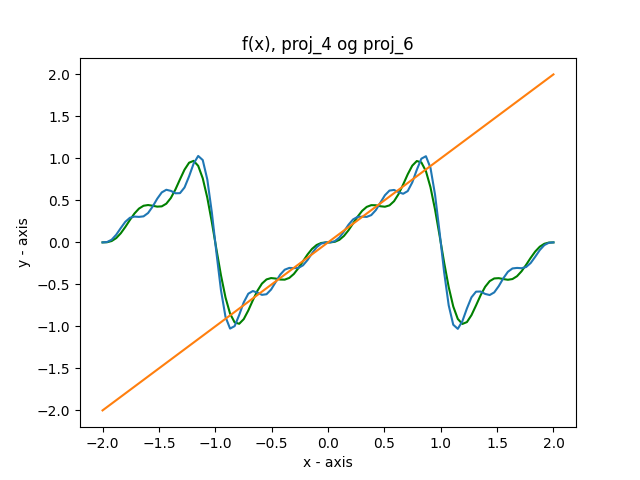
\includegraphics[width=0.7\textwidth]{opg2h.png}\\

    \newpage



    \section{Oppgave}

    fil: kabal.py


\end{document}
